% Presentación para la sustentación (15 diapositivas, ~15 minutos). Compilar: ./tectonic.exe presentacion.tex
\documentclass[aspectratio=169,11pt]{beamer}
\usepackage{fontspec}
\usepackage[spanish,es-nodecimaldot,es-noshorthands]{babel}
\usepackage{booktabs}
\graphicspath{{../notebooks/resultados/figuras/}}

\definecolor{azul}{HTML}{1F3A5F}
\definecolor{gris}{HTML}{6B7280}
\setbeamercolor{frametitle}{fg=azul}
\setbeamercolor{title}{fg=azul}
\setbeamercolor{structure}{fg=azul}
\setbeamerfont{frametitle}{series=\bfseries,size=\Large}
\setbeamertemplate{navigation symbols}{}
\setbeamertemplate{footline}{\hfill{\scriptsize\color{gris}\insertframenumber/\inserttotalframenumber}\hspace{1em}\vspace{0.6em}}
\setbeamertemplate{itemize items}[circle]
\newcommand{\dato}[2]{\begin{minipage}[t]{0.42\linewidth}\centering{\Huge\bfseries\color{azul}#1}\\[2pt]{\small #2}\end{minipage}}

\title{Efecto causal de la cochera incluida en el precio de oferta de alquiler en Lima Metropolitana}
\subtitle{Inferencia causal espacial asistida por inteligencia artificial}
\author{Luis Azaña}
\institute{Seminario de Tesis 2}
\date{2026}

\begin{document}

\begin{frame}
\titlepage
\end{frame}

% 2 -----------------------------------------------------------------
\begin{frame}{Problema: la correlación no responde la pregunta}
\begin{columns}[T]
\column{0.55\textwidth}
\begin{itemize}
\item Pregunta contrafactual: \textbf{¿cuánto cambiaría el alquiler si el mismo departamento incluyera cochera?}
\item Los departamentos con cochera son también más grandes (96 vs 65\,m²) y están en zonas más caras.
\item La cochera \textbf{no es un campo de la base}: está en el texto del aviso.
\item Los estudios locales \textbf{predicen} precios (hedónico, XGBoost); no identifican efectos.
\end{itemize}
\column{0.42\textwidth}
\vspace{0.8cm}
\begin{center}
\dato{+63\%}{diferencia\\sin ajustar}\hspace{0.5em}\dato{?}{efecto\\causal}
\end{center}
\end{columns}
\end{frame}

% 3 -----------------------------------------------------------------
\begin{frame}{Alcance, objetivos e hipótesis}
\begin{columns}[T]
\column{0.5\textwidth}
\textbf{Alcance}
\begin{itemize}\small
\item Precio \emph{de oferta} mensual, no contrato.
\item Avisos de un portal, 13 distritos, marzo 2025, \textbf{solo direcciones exactas (ROOFTOP)}.
\item Tratamiento: cochera incluida (sí/no). Secundario: nº de baños.
\end{itemize}
\textbf{Objetivos}
\begin{itemize}\small
\item OE1 auditoría · OE2 identificación · OE3 estimación
\item OE4 heterogeneidad y sensibilidad · OE5 medición con IA
\item OE6 simulación · OE7 trazabilidad
\end{itemize}
\column{0.47\textwidth}
\textbf{Hipótesis} (sin dirección obligatoria)
\begin{itemize}\small
\item H1: el ajuste cambia la asociación.
\item H2: los controles importan más que el algoritmo.
\item H3: el efecto varía por zona o tamaño (si la precisión lo respalda).
\item H4: la solidez depende de los confusores no observados.
\end{itemize}
\end{columns}
\end{frame}

% 4 -----------------------------------------------------------------
\begin{frame}{Datos: auditoría de la muestra (R1)}
\begin{columns}[T]
\column{0.44\textwidth}
\footnotesize
\begin{tabular}{@{}lr@{}}
\toprule
Paso & N \\
\midrule
Archivo crudo & 3\,739 \\
Variables núcleo completas & 3\,516 \\
\textbf{$-$ duplicados} & $-$243 \\
$-$ geocodificación incoherente & $-$26 \\
\textbf{$-$ dirección no exacta} & $-$967 \\
$-$ reglas de depuración & $-$60 \\
\midrule
\textbf{Muestra analítica} & \textbf{2\,220} \\
\bottomrule
\end{tabular}

\vspace{0.3cm}
\footnotesize La ubicación es el confusor más fuerte: solo se usan direcciones con el edificio exacto. Con todas las precisiones, el efecto de los baños se inflaba (5.1 vs 3.8\,\%).
\column{0.54\textwidth}
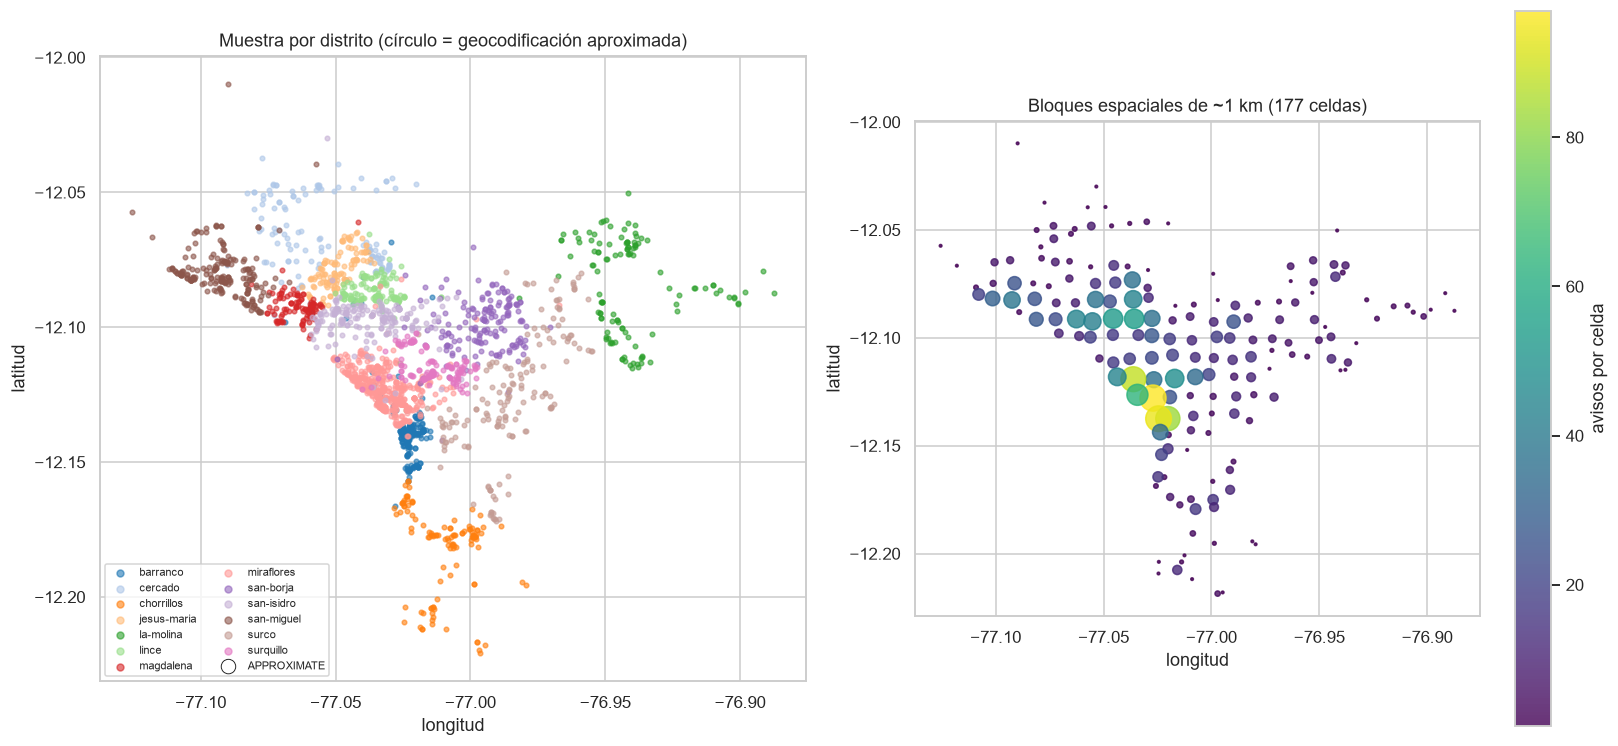
\includegraphics[width=\textwidth]{F2_territorio.png}
\end{columns}
\end{frame}

% 5 -----------------------------------------------------------------
\begin{frame}{Medición de la cochera con IA (OE5)}
\begin{columns}[T]
\column{0.52\textwidth}\small
\begin{enumerate}
\item \textbf{Regex}: ¿menciona cochera/estacionamiento? Si no $\rightarrow$ sin cochera (659 avisos, sin costo).
\item \textbf{Fragmento} \texttt{texto[x-200:x+200]}; se enmascaran teléfonos y correos.
\item \textbf{gpt-4.1-mini}, temperatura 0, JSON fijo:\\
{\scriptsize\texttt{\{"cochera":"si", "precio\_extra":0, \ldots\}}}
\item Piloto de 25 avisos: se corrigieron 3 errores del prompt.
\end{enumerate}
\textbf{Costo total: 0.76 USD} (1\,561 avisos enviados).
\column{0.46\textwidth}\small
\begin{tabular}{lr}
\toprule
Clasificación & N \\
\midrule
Cochera incluida ($D=1$) & 1\,095 \\
Sin mención ($D=0$) & 659 \\
``No tiene'' según la IA ($D=0$) & 297 \\
Costo extra (excluido) & 150 \\
Ambigua (excluido) & 19 \\
\bottomrule
\end{tabular}

\vspace{0.3cm}
\footnotesize Validación humana: 249 avisos preparados, \textbf{pendiente}.
\end{columns}
\end{frame}

% 6 -----------------------------------------------------------------
\begin{frame}{Intervención, estimando y DAG}
\begin{columns}[T]
\column{0.6\textwidth}
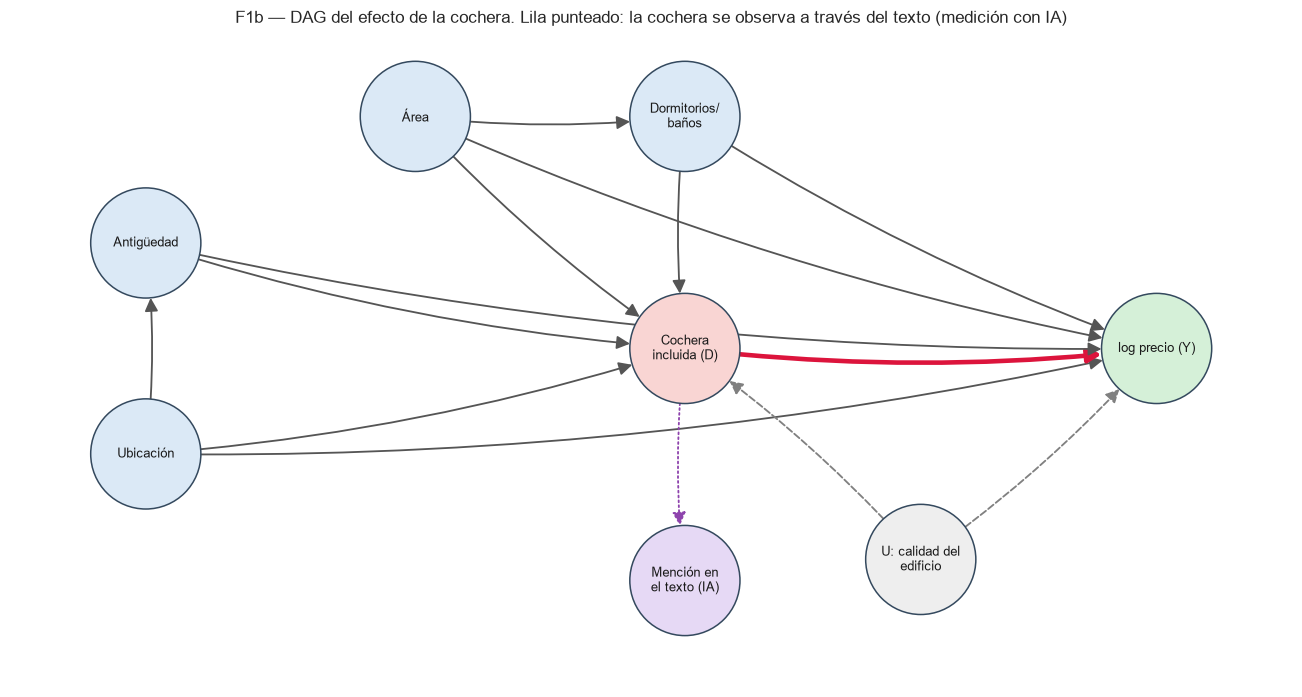
\includegraphics[width=\textwidth]{F1b_dag_cochera.png}
\column{0.38\textwidth}\small
\begin{itemize}
\item \textbf{Estimando}: ATE de tener cochera incluida, en la población con soporte común (propensión 0.05--0.95).
\item \textbf{Ajustar}: área, dormitorios, baños, antigüedad, ubicación.
\item \textbf{No ajustar}: precio/m² (descendiente de $Y$).
\item \textbf{Amenaza}: calidad del edificio ($U$) y error de medición del texto.
\end{itemize}
\end{columns}
\end{frame}

% 7 -----------------------------------------------------------------
\begin{frame}{Método: Double ML interactivo (IRM / AIPW)}
\begin{enumerate}
\item \textbf{Propensión} $m(X)=P(\text{cochera}\mid X)$ con un clasificador de \textit{gradient boosting}.
\item \textbf{Resultado} $g_1(X)$, $g_0(X)$: precio esperado con y sin cochera (un modelo por grupo).
\item \textit{Cross-fitting} con 5 folds \textbf{agrupados por edificio} $\times$ 10 repeticiones.
\item Score doblemente robusto, promediado en el soporte común:
\[\phi=g_1-g_0+\frac{D(Y-g_1)}{m}-\frac{(1-D)(Y-g_0)}{1-m}\]
\item Inferencia \textbf{agrupada por edificio} (alternativa: bloques de 1\,km).
\end{enumerate}
\vspace{0.2cm}
\small Además: soporte común y balance, grilla de especificaciones, sensibilidad, GATE, I de Moran y simulación.
\end{frame}

% 8 -----------------------------------------------------------------
\begin{frame}{Soporte común y balance (R2)}
\centering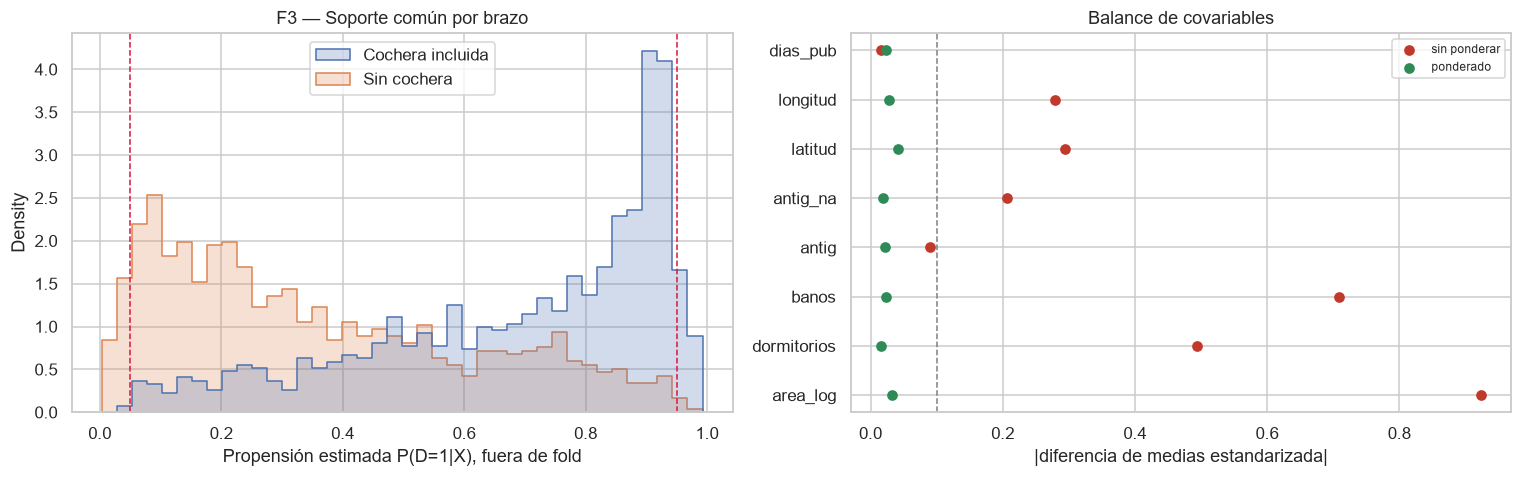
\includegraphics[height=0.5\textheight]{F3_soporte_cochera.png}\par
\small
\begin{itemize}
\item AUC de la propensión = 0.82; solo el \textbf{5\,\%} de los avisos queda fuera de [0.05, 0.95] (1\,949 en soporte común).
\item Antes de ponderar: diferencias de 0.92 (área) y 0.71 (baños). Después: todas $<0.05$ $\rightarrow$ grupos comparables.
\end{itemize}
\end{frame}

% 9 -----------------------------------------------------------------
\begin{frame}{Resultado principal (R3)}
\begin{columns}[c]
\column{0.36\textwidth}
\begin{center}
{\Huge\bfseries\color{azul} +7.5\%}\\[4pt]
{\small por tener cochera incluida}\\[2pt]
{\small IC 95\,\%: 3.7 -- 11.4\,\%}\\[10pt]
{\Large\bfseries\color{azul} $\approx$ S/ 199}\\[2pt]
{\small al mes (alquiler de S/ 2\,650)}
\end{center}
\column{0.62\textwidth}
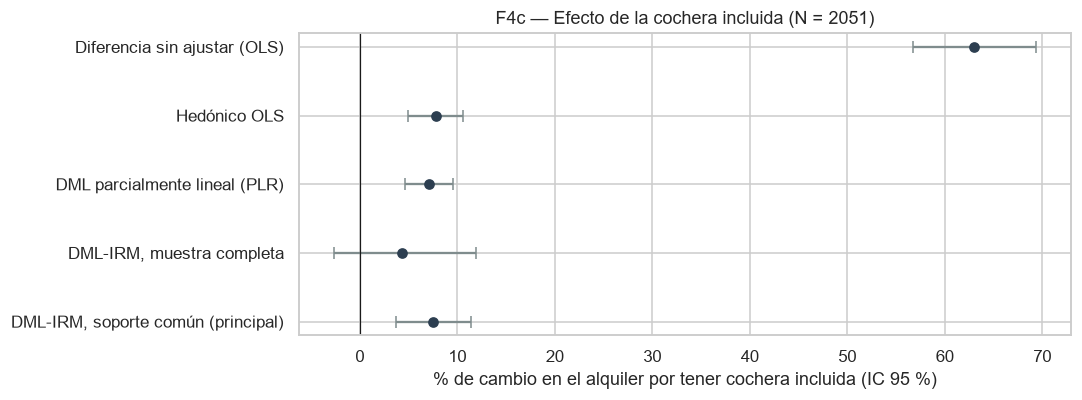
\includegraphics[width=\textwidth]{F4c_estimadores_cochera.png}
\end{columns}
\vspace{0.2cm}
\footnotesize Sin ajustar: 63\,\% $\rightarrow$ hedónico 7.8\,\% · PLR 7.1\,\% · IRM 7.5\,\%. Sin recorte, el IRM es inestable (IC de $-2.7$ a 11.9\,\%). \textbf{H1 se confirma.}
\end{frame}

% 10 ----------------------------------------------------------------
\begin{frame}{¿Qué decisiones importan? (R4)}
\begin{columns}[c]
\column{0.5\textwidth}\small
\begin{tabular}{lr}
\toprule
Especificación & Efecto \\
\midrule
Principal & 7.6\,\% \\
Sin ubicación & \textbf{21.7\,\%} \\
Sin área & 11.4\,\% \\
Sin baños ni dormitorios & 9.1\,\% \\
+ precio/m² (prohibido) & $-0.5$\,\% \\
Solo ``incluida'' explícita & 7.9\,\% \\
Costo extra también tratado & 5.3\,\% \\
Bloques de 1\,km & 7.7\,\% \\
\bottomrule
\end{tabular}
\column{0.48\textwidth}\small
\begin{itemize}
\item Las cocheras abundan en distritos caros: \textbf{sin ubicación el efecto se triplica}.
\item El control prohibido lo anula.
\item Las alternativas de medición se mueven en la dirección esperada.
\end{itemize}
\textbf{H2 se confirma}.
\end{columns}
\end{frame}

% 11 ----------------------------------------------------------------
\begin{frame}{Heterogeneidad: la cochera vale más donde escasea (R7)}
\centering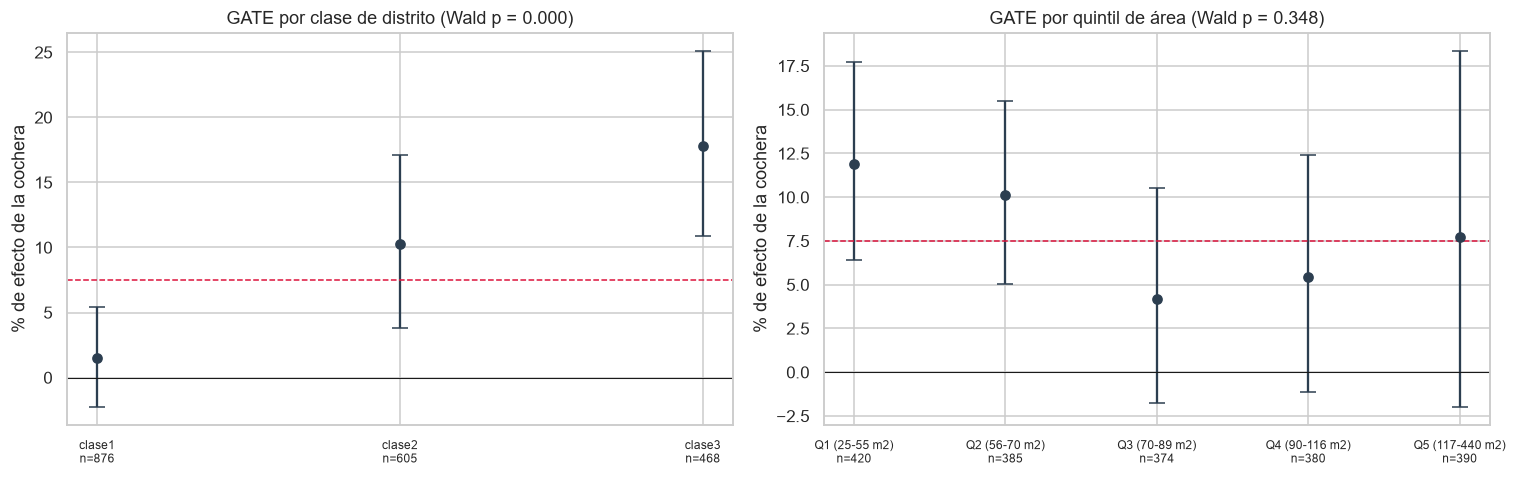
\includegraphics[height=0.52\textheight]{F7c_heterogeneidad_cochera.png}\par
\small
\begin{itemize}
\item Miraflores, San Isidro, Barranco, Lince: \textbf{1.5\,\%} (n.s.) · clase2: \textbf{10\,\%} · clase3: \textbf{18\,\%}. Wald $p=0.0001$ $\rightarrow$ \textbf{H3 se confirma}.
\item Interpretación (hipótesis): donde casi todos los avisos tienen cochera, no se paga extra por ella.
\end{itemize}
\end{frame}

% 12 ----------------------------------------------------------------
\begin{frame}{Robustez a confusores no observados (R5)}
\begin{columns}[c]
\column{0.5\textwidth}
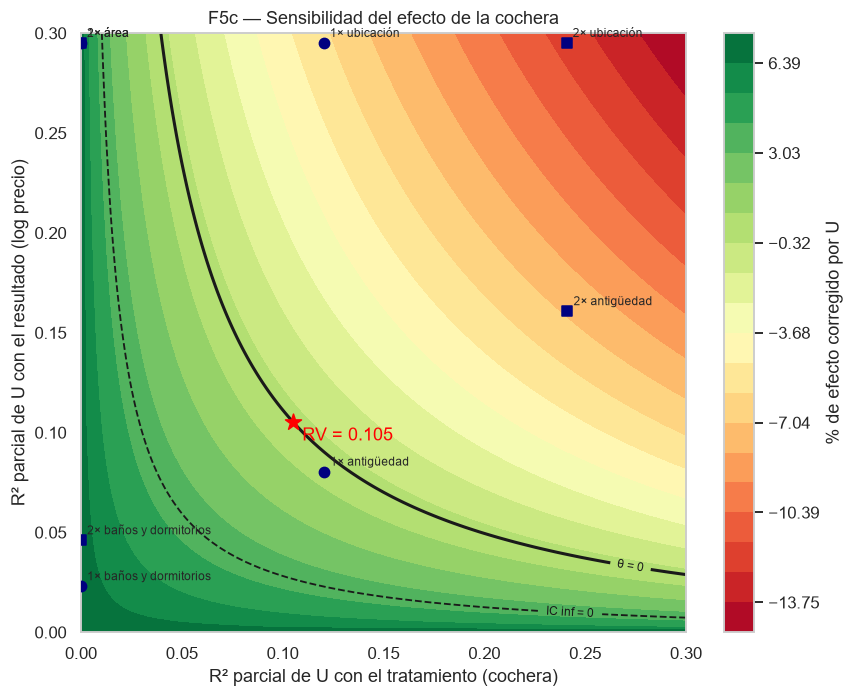
\includegraphics[width=\textwidth]{F5c_sensibilidad_cochera.png}
\column{0.48\textwidth}\small
\begin{itemize}
\item \textbf{RV = 0.105}: un $U$ que explique el 10.5\,\% de la variación residual de la cochera \emph{y} del precio anula el efecto.
\item $U$ tan fuerte como la \textbf{antigüedad} $\rightarrow$ 0.4\,\%.
\item $U$ tan fuerte como la \textbf{ubicación} $\rightarrow$ signo negativo.
\item La simulación muestra que esta cota es \textbf{optimista}: la fragilidad podría ser mayor.
\end{itemize}
\textbf{H4 se confirma}: resultado frágil.
\end{columns}
\end{frame}

% 13 ----------------------------------------------------------------
\begin{frame}{Validación semisintética (R6) y análisis de baños}
\begin{columns}[T]
\column{0.5\textwidth}\small
\textbf{Simulación} (800 réplicas, covariables reales)
\begin{itemize}
\item \textbf{Cochera sin $U$}: los tres métodos aciertan (cobertura 94--96\,\%).
\item \textbf{Cochera con $U$}: todos se sesgan ($+0.04$); la cota subestima el sesgo.
\item \textbf{Baños sin $U$}: DML insesgado; el hedónico lineal sobreestima.
\item \textbf{Baños con $U$}: la cota sí funciona (cobertura 95--98\,\%).
\end{itemize}
\column{0.48\textwidth}\small
\textbf{Un baño adicional} (secundario)
\begin{itemize}
\item \textbf{+3.8\,\%} (1.7--6.0\,\%) $\approx$ S/ 100 al mes.
\item Controlando por cochera: 3.5\,\%.
\item Con direcciones imprecisas subía a 5.1\,\%.
\item Sin heterogeneidad; frágil frente a un $U$ como la antigüedad.
\end{itemize}
\end{columns}
\end{frame}

% 14 ----------------------------------------------------------------
\begin{frame}{Conclusiones y límites}
\begin{itemize}
\item \textbf{Respuesta}: bajo los supuestos del DAG, tener cochera incluida eleva el precio de oferta en \textbf{7.5\,\%} (3.7--11.4\,\%), unos S/\,199 al mes; casi nada en los distritos más caros y hasta 18\,\% donde escasea.
\item \textbf{Observacional}: casi todo el 63\,\% bruto es tamaño y zona.
\item \textbf{Metodológico}: la IA permite medir un atributo del texto por menos de 1 USD; la geocodificación exacta cambia los resultados.
\item \textbf{Límites}: confusor de calidad del edificio, medición con IA sin validación humana, cota de sensibilidad optimista, un portal y un mes.
\item \textbf{No se afirma}: que agregar una cochera sea rentable, ni que valga para contratos o para toda Lima.
\end{itemize}
\end{frame}

% 15 ----------------------------------------------------------------
\begin{frame}{Contribución y continuidad}
\begin{columns}[T]
\column{0.48\textwidth}
\textbf{Contribución verificable}
\begin{itemize}\small
\item Auditoría reproducible (duplicados, precisión de la dirección).
\item Medición barata y trazable de atributos con IA.
\item Efecto con soporte común, balance e inferencia agrupada.
\item Evidencia de heterogeneidad por escasez.
\end{itemize}
\column{0.48\textwidth}
\textbf{Siguiente paso}
\begin{itemize}\small
\item Validación humana de 249 avisos.
\item Medir la calidad del edificio desde el texto.
\item Mejorar la cota de sensibilidad binaria.
\item Repositorio con una orden reproducible.
\end{itemize}
\end{columns}
\vspace{0.6cm}
\begin{center}\Large\color{azul}\textbf{¡Gracias!}\end{center}
\end{frame}

\end{document}
